\documentclass[11pt]{article}
\usepackage{fullpage,amsmath,amsfonts,mathpazo,microtype,nicefrac,graphicx}

% Set-up for hypertext references
\usepackage{hyperref,color,textcomp}
\definecolor{webgreen}{rgb}{0,.35,0}
\definecolor{webbrown}{rgb}{.6,0,0}
\definecolor{RoyalBlue}{rgb}{0,0,0.9}
\hypersetup{
   colorlinks=true, linktocpage=true, pdfstartpage=3, pdfstartview=FitV,
   breaklinks=true, pdfpagemode=UseNone, pageanchor=true, pdfpagemode=UseOutlines,
   plainpages=false, bookmarksnumbered, bookmarksopen=true, bookmarksopenlevel=1,
   hypertexnames=true, pdfhighlight=/O,
   urlcolor=webbrown, linkcolor=RoyalBlue, citecolor=webgreen,
   pdfauthor={Chris H. Rycroft},
   pdfsubject={Harvard AM205 (Fall 2017)},
   pdfkeywords={},
   pdfcreator={pdfLaTeX},
   pdfproducer={LaTeX with hyperref}
}
\hypersetup{pdftitle={AM205: Final Project}}

% Macro definitions
\newcommand{\N}{\mathbb{N}}
\newcommand{\Z}{\mathbb{Z}}
\newcommand{\Q}{\mathbb{Q}}
\newcommand{\R}{\mathbb{R}}
\newcommand{\B}{\mathbb{B}}
\newcommand{\mcL}{\mathcal{L}}
\newcommand{\p}{\partial}
\newcommand{\Trans}{\mathsf{T}}
\renewcommand{\vec}[1]{\mathbf{#1}}
\newcommand{\vx}{\vec{x}}
\newcommand{\vb}{\vec{b}}

% ====== shortcut =======
\newcommand{\nn}{neural network}
\newcommand{\ann}{artificial neural network}
\newcommand{\Ann}{Artificial neural network}

\DeclareMathOperator{\rank}{rank}
\title{AM205: Final Project Report}
\author{Jiawei Zhuang, Xu Si, Rui Zhao, Chin Hui Chew}
\date{December 2017}

\begin{document}

\maketitle

\section{Introduction}

(to add: application of ODEs, e.g. population growth, chemical kinetics) \\

Ordinary differential equations (ODEs) are generally solved by finite-differencing methods, from the simplest forward Euler scheme to higher-order schemes like the Runge-Kutta methods. Numerical solutions obtained by those schemes are typically stored in a discretized form, i.e. in an array of floating point numbers. \\

The \ann\ (ANN) method \cite{Lagaris98} provides an way to obtain ODE solutions in a closed analytical form. The solutions are stored as \nn\ parameters, which requires much less memory than storing the solution as a discretized array. Also, because the solution is analytically differentiable, it can be superior in some applications like sensitivity analysis.

\section{Method}

\subsection{Fitting functions by artificial neural networks}

The universal approximation theorem \cite{Hornik89} states that any continuous function can be approximated by a feed-forward \nn\ with a single hidden layer. This ANN can be written in a matrix multiplication form:

\begin{equation}
N(x; w) = W_2 \sigma(W_1 x + b_1) + b_2
\end{equation}

where $W_1$ and $W_2$ are weight matrices and $b_1$ and $b_2$ are bias terms. $\sigma$ is a nonlinear activation function such as $tanh$. We use $w$ to represent all parameters [$W_1$, $W_2$, $b_1$, $b_2$]. 
\\

To fit a scalar function $y(x)$, the \nn\ takes a scalar input $x$ and returns a scalar output $N(x)$. In this case, $W_1$ and $W_2$ degrade to row and column vectors.
\\

The optimal parameters $w$ can be found by minimizing the loss function
\begin{equation}
L(w) = \int_a^b [y(x)-N(x; w)]^2 dx
\end{equation}

In practice, the integral is approximated by a summation
\begin{equation}
L(w) = \sum_i [y(x_i)-N(x_i; w)]^2
\end{equation}
where \{$x_i$\}  is a set of training points covering the domain [$a$, $b$]. 
\\

If the loss is small enough, then the ANN can be considered as a good approximation to the original function over the domain the domain [$a$, $b$]:
\begin{equation}
N(x; w) \approx y(x)
\end{equation}

% ------- a new subsection -------
\subsection{Solving one ODE by \ann s}

Now we consider constructing an ANN that can approximate the solution to the first-order ODE:
\begin{equation}
y'(t) = F(y(t), t), \ \ y(t_0)=y_0
\end{equation}

If we use a standard \nn
\begin{equation}
N(t; w) = W_2 \sigma(W_1 t + b_1) + b_2
\end{equation}

It will not satisfy the initial condition, i.e. typically $N(t_0; w) \ne y_0$. But we can force the initial condition by rewriting the ANN solution as
\begin{equation}
\hat{y}(t; w) = y_0 + (t-t_0) N(t; w)
\end{equation}

For any parameters $w$, there will always be $\hat{y}(t_0; w) = y_0$. We further require this ANN solution $\hat{y}(t; w)$ to satisfy the ODE:

\begin{equation}
\hat{y}'(t; w) \approx F(\hat{y}(t; w), t)
\end{equation}

Note that the derivative $\hat{y}'(t; w)$ can be derived analytically without any finite-difference approximation
\begin{equation}
\hat{y}'(t; w)
= \frac{\partial[y_0+(t-t_0) N(t; w)]}{\partial t}
= \frac{\partial(t-t_0)}{\partial t}N(t; w) + (t-t_0)\frac{\partial N(t; w)}{\partial t}
\end{equation}

The optimal parameters can be found by minimizing the cost function
\begin{equation}
L(w) = \int_{t_0}^{t_1} [ \hat{y}'(t; w) - F(\hat{y}(t; w), t) ] ^ 2 dt
\end{equation}

Or in practice, 
\begin{equation}
L(w) \approx \sum_i [ \hat{y}'(t_i; w) - F(\hat{y}(t_i; w), t_i) ] ^ 2
\end{equation}
where \{$t_i$\} is a set of training points covering the domain [$t_0$, $t_1$].
\\

If the loss is small enough, then the ANN solution should be able to approximate the true ODE solution over the domain [$t_0$, $t_1$]:
\begin{equation}
\hat{y}(t; w) \approx y(t)
\end{equation}

% ------- a new subsection -------
\subsection{Solving ODE systems by \ann s}

The above ANN method can be directly generalize to a system of ODEs. For simplicity, consider two ODEs
\begin{align}
y'(t) = F_1(y(t), z(t), t), \ \ y(t_0)=y_0 \\
z'(t) = F_2(y(t), z(t), t), \ \ z(t_0)=z_0
\end{align}

We can use two separates ANNs for two variables $y$ and $z$
\begin{align}
\hat{y}(t; w) = y_0 + (t-t_0) N_1(t; w_1) \\
\hat{z}(t; w) = z_0 + (t-t_0) N_2(t; w_2)
\end{align}

Then loss function is the sum of losses for two ODEs
\begin{equation}
L(w_1, w_2) \approx \sum_i
\Big[
[\hat y'(t_i) - F_1(\hat y(t_i), \hat z(t_i), t_i)]^2
+
[\hat z'(t_i) - F_2(\hat y(t_i), \hat z(t_i), t_i)]^2
\Big]
\end{equation}


\section{Results and Discussions}

In this section, we will apply the \Ann method to four common types of ODE problems: (1)simple ODE, (2)unstable and periodic ODE, (3)unstable and chaotic ODE and (3)stiff ODE system and then compare Neural Network results with traditional finite difference method which we treat as ground truth. We have found that in most cases, ANN method can approximate the ground truth well, whereas sometimes we need to train the network multiple times to get ideal results. Also, our method only works for a given range of data, yielding unreliable fits in extrapolation. 

In all the examples, we train our ANN using BFGS whose performance of convergence out beats all other optimisers. We also compare ground truth and ANN fit both in the training domain and outside domain. To test the stability of our ANN method, we retrain the ANN 100 times and plot average RMSE

\subsection{Simple ODEs}
\textbf{Overview}

Consider a first-order ODE system:
    \begin{equation}
      \frac{dx}{dt} = \cos t+x^2 + y - (1 + t^2 +\sin^2t)
      \label{eq:simple_eq1}
    \end{equation}
    
     \begin{equation}
      \frac{dy}{dt} = 2t - (1 + t^2)\sin t + xy
      \label{eq:simple_eq2}
    \end{equation}

    
where $t \in [0, 3]$.

\textbf{Mathematics}

The analytical solutions are:
    \begin{equation}
      x = \sin t
      \label{eq:simple_eq3}
    \end{equation}
    
     \begin{equation}
      y= 1 + x^2
      \label{eq:simple_eq4}
    \end{equation}

Ideally, our NN solver should attain the same solution as the exact analytical solutions within the time range specified.

\textbf{Results}

The solutions using the Neural Net solver could be found in Fig.~\ref{fig:SimpleFig}. The network was trained using a grid of 20 equidistant points in $t = [0, 3]$ and 50 hidden units in the hidden layer. 

\begin{figure}
\centering
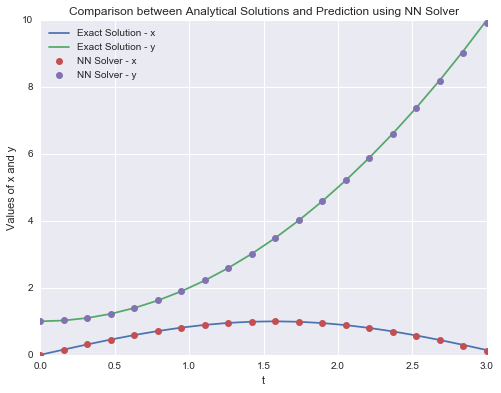
\includegraphics[width=0.7\textwidth]{result_simple.png}
      \caption{Comparing solutions found using neural net solver versus exact analytical solutions. Average RMSE = 0.0524. \label{fig:SimpleFig}}
\end{figure}

We could see almost an exact fit with the analytical solution. In terms of training convergence, we could see that the neural net rapidly converges to a solution with log loss value of order $10^{-4}$ at 200 iterations from Fig. ~\ref{fig:SimpleLoss}. BFGS is selected as the optimization method because it results in the lowest loss at 200 iterations.

\begin{figure}
\centering
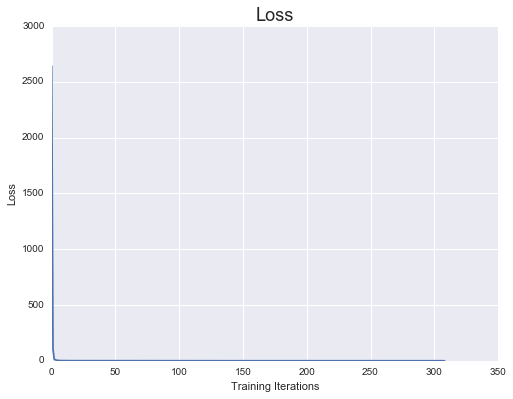
\includegraphics[width=0.7\textwidth]{loss_simple.png}
      \caption{Comparison across different optimization methods for simple ODE system. \label{fig:SimpleLoss}}
\end{figure}

\textbf{Discussions}

To enable us to evaluate the fit of the two functions in this system of ODE, we propose taking an average of the RMSE, in this case we will have:

\begin{equation}
RMSE_{overall} = \frac{1}{2}[RMSE_{x} + RMSE_{y}]
\end{equation}

The fitting attained as shown in Fig. \ref{fig:SimpleFig} has $RMSE_{overall} = 0.0524$.

Note that average RMSE enables us to determine the reproducibility of a good performing model for the same ODE system, but it is not necessary a good metrics to compare the fit for different ODE systems. 

In terms of reproducibility, we repeated the same fitting process 100 times. The average RMSE histogram distribution for 100 fittings is shown in Fig. \ref{fig:SimpleHistogram}. 55\% of the fittings are relatively close fit to the exact analytical solution, with RMSE of up to 0.0378, while our plot in Fig.~\ref{fig:SimpleFig} has RMSE = 0.0524.

\begin{figure}
\centering
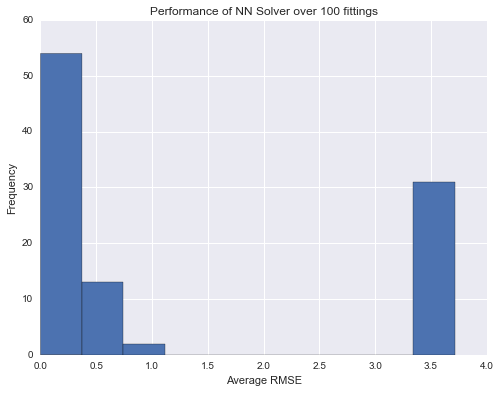
\includegraphics[width=0.7\textwidth]{histogram_simple.png}
      \caption{Average RMSE Distribution for 100 Repeated Fittings for Simple ODE System. \label{fig:SimpleHistogram}}
\end{figure}

Please refer to SimpleODE.ipynb for the code and visualizations of this section.

\subsection{Lotka-Volterra 2-species model}
\textbf{Overview}

The Lotka-Volterra prey-predator equations are a pair of first-order, non-linear differential equations commonly used to describe the interactions between two species, the prey and predator.

\textbf{Mathematics}

The populations of the prey and predator can be described by the following equations:

    \begin{equation}
      \frac{dx}{dt} = ax - bxy
      \label{eq:LV1}
    \end{equation}
    
     \begin{equation}
      \frac{dy}{dt} = -cy + dxy
      \label{eq:LV2}
    \end{equation}
    

where
\begin{itemize}
\item $x$ is the density of prey
\item $y$ is the density predator
\item $t$ represents time
\item $a, b, c, d >0$ 
\end{itemize}

Eq.~\ref{eq:LV1} indicates that in the absence of a predator ($y = 0$), the prey would grow at a constant rate $a$, with the assumption that the prey have an unlimited food supply. The rate of predation upon the prey is assumed to be proportional to the rate at which the predators and the prey are present concurrently, represented by $bxy$. If either $x$ or $y$ is zero then no predation is possible.

Similarly, Eq.~\ref{eq:LV2} shows that in the absence of prey ($x = 0$), the density of predators would decrease at a constant rate $c$, due to natural death or emigration. This equation assumes that the predator population only preys upon the same species of prey identified in Eq.~\ref{eq:LV1}. $dxy$ represents the growth of the predator population~\cite{REF1}.

The model assumes that throughout the process the external environment remains the same and none of the species is favored~\cite{REF2}.

\textbf{Results}

\begin{figure}
\centering
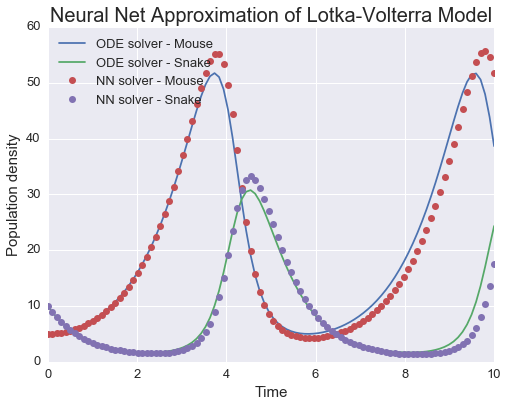
\includegraphics[width=0.7\textwidth]{LV_Compare.png}
      \caption{Comparing across results using standard ODE solver from Scipy library versus using neural net solver, at initial parameters of $a = 1$, $b = 0.1, c = 1.5, d = 0.75$. Average RMSE = 2.204. \label{fig:LVFig}}
\end{figure}

\begin{figure}
\centering
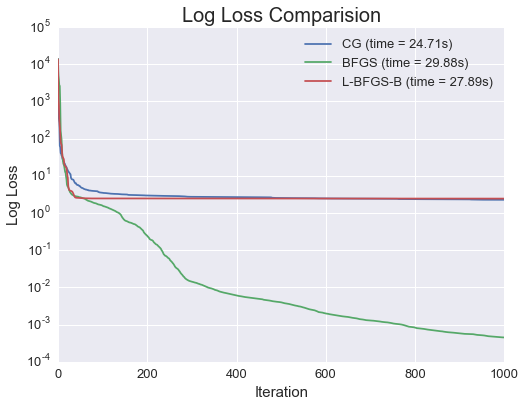
\includegraphics[width=0.7\textwidth]{lossMethod_LV.png}
      \caption{Convergence to final solutions for 2-species model \label{fig:loss_LV2}}
\end{figure}

From Fig.~\ref{fig:LVFig} we see that our neural net solver attains a close fit to the ODE solver. Training was done with a grid of 100 equidistant points in $t = [0, 10]$ and 50 hidden units in the hidden layer. 

In terms of training convergence, from Fig. \ref{fig:loss_LV2}, we can see that BFGS is selected as the optimization method as it results in the lowest loss compared to other methods.

\textbf{Discussions}

The same as before, to enable us to evaluate the fit of the two functions in this system of ODEs, we propose taking an average of the RMSE, in this case we will have:

\begin{equation}
RMSE_{overall} = \frac{1}{2}[RMSE_{prey} + RMSE_{predator}]
\end{equation}

For this particular plot, the overall average RMSE is at $2.204$. It is found that while our proposed solver using neural net is able to provide a continuous function, the results tend to fluctuate highly. As such, we ran the same fitting over 100 times as shown in Fig. ~\ref{fig:perf_dist}. 32\% of the fittings result in relatively good fitting with average RMSE of less than 5.

Please refer to LV2.ipynb for the code and visualizations of this section.

\begin{figure}
\centering
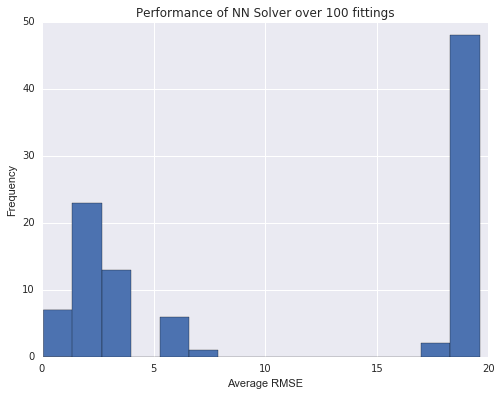
\includegraphics[width=0.7\textwidth]{perf_distribution.png}
      \caption{Running NN solver 100 times to see the performance histogram \label{fig:perf_dist}}
\end{figure}


\subsection{Lotka-Volterra 3-species Model}
Extending to the 2-species model discussed earlier, we wish to model a linear three-species food chain where the lowest-level prey $x$ is preyed upon by a mid-level species $y$, which, in turn, is preyed upon by a top level predator $z$. An example of a three-species food chain is mouse-snake-owl~\cite{REF3}.  

    \begin{equation}
      \frac{dx}{dt} = ax - bxy
      \label{eq:LV3}
    \end{equation}
    
     \begin{equation}
      \frac{dy}{dt} = - cy + dxy - eyz
      \label{eq:LV4}
    \end{equation}
    
     \begin{equation}
      \frac{dz}{dt} = - fz + gyz
      \label{eq:LV5}
    \end{equation}
where
\begin{itemize}
\item $a, b, c, d, e, f, g >0$ 
\item $a, b, c, d$ are as in the 2-species Lotka-Volterra equations
\item $e$ represents the effect of predation on species $y$ by species $z$
\item $f$ represents the natural death rate of species $z$ in the absence of prey
\item $g$ represents the reproduction rate of species $z$ in the presence of prey $y$
\end{itemize}

\textbf{Results}


\begin{figure}
\centering
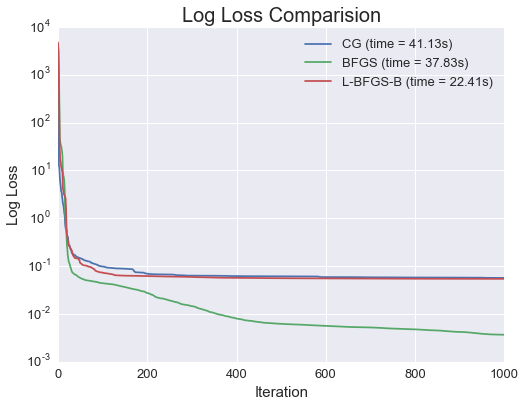
\includegraphics[width=0.7\textwidth]{lossMethod_LV3.png}
      \caption{Convergence to final solutions for 3-species model \label{fig:loss_LV3}}
\end{figure}

\begin{figure}
\centering
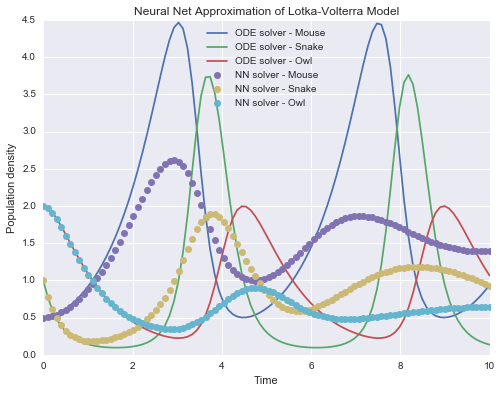
\includegraphics[width=0.7\textwidth]{LV_Compare_3_species.png}
      \caption{Comparing across results using standard ODE solver from Scipy library versus using neural net solver, at initial parameters of $a = b = c = d = e = f = g = 1 $. Average RMSE score of 0.803. \label{fig:LVFig_3_species}}
\end{figure}

The neutral net is trained with 50 hidden units over 100 equidistant points over $t \in [0, 10]$. As before, the optimization method is BFGS because the log loss is the smallest compared to other methods at the 200 iterations as shown in Fig.~\ref{fig:loss_LV3}. 

From Fig.~\ref{fig:LVFig_3_species}, we can see that the performance is worse compared to the 2-species Lotka-Volterra model. The fit is close to the solution from ODE solver only up to $t = 2.5$ for the three equations. No further model fitting is carried out to examine reproducibility as the fitting is poor and the average RMSE score is not a good gauge to identify strong fit. 

Please refer to LV3.ipynb for the code and visualizations of this section.

\subsection{Van der Pol oscillator}
\textbf{Overview}

Van der Pol oscillator is a non-conservative oscillator with a linear spring force and a non-linear damping force~\cite{REF4}. The equation is given by:
     \begin{equation}
      \frac{d^2x}{dt^2} - \mu(1-x^2)\frac{dx}{dt} + x = 0
      \label{eq:VDP}
    \end{equation}
    
\textbf{Mathematics}

Applying the Li\'enard transformation $y = x - \frac{x^3}{3} - \frac{1}{\mu}\frac{dx}{dt}$, the equation can be written as a system of ODE ~\cite{REF5}:

     \begin{equation}
      \frac{dx}{dt} = \mu(x - \frac{1}{3}x^3 - y)
      \label{eq:VDP1}
    \end{equation}
    
     \begin{equation}
      \frac{dy}{dt} = \frac{x}{\mu}
      \label{eq:VDP2}
    \end{equation}
    
\textbf{Results}

\begin{figure}
\centering
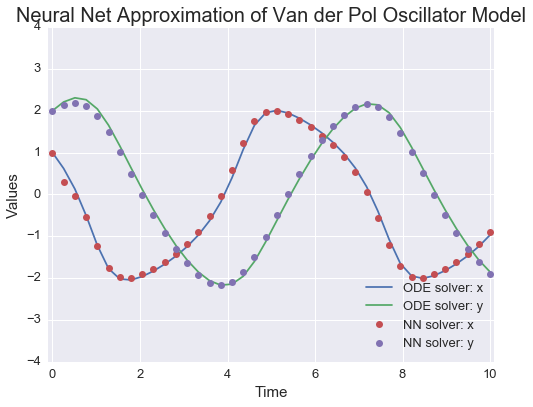
\includegraphics[width=0.7\textwidth]{VDP_uniform_good.png}
      \caption{Running NN solver with even spacing on time points. Average RMSE of 0.0999. \label{fig:VDP_uniform}}
\end{figure}

From Fig.~\ref{fig:VDP_uniform} we see that our neural net solver attains a close fit to the ODE solver. Training was done with a grid of 40 equidistant points in $t = [0, 10]$ and 20 hidden units in the hidden layer. BFGS is used as the optimization method as we could see from Fig.~\ref{fig:loss_VDP} that the method attains the lowest log loss.

\begin{figure}
\centering
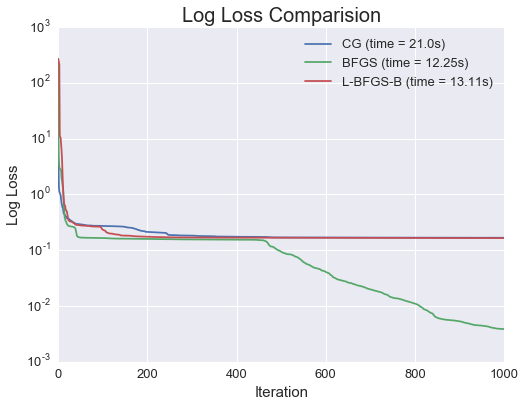
\includegraphics[width=0.7\textwidth]{lossMethod_VDP.png}
      \caption{Convergence to final solutions for VDP. \label{fig:loss_VDP}}
\end{figure}

\textbf{Discussions}

The same as before, to evaluate the fit of the two functions in this system of ODEs, we propose taking an average of the RMSE, in this case the overall average RMSE for our fit in Fig.~\ref{fig:VDP_uniform} is at $0.0999$. 

\begin{figure}
\centering
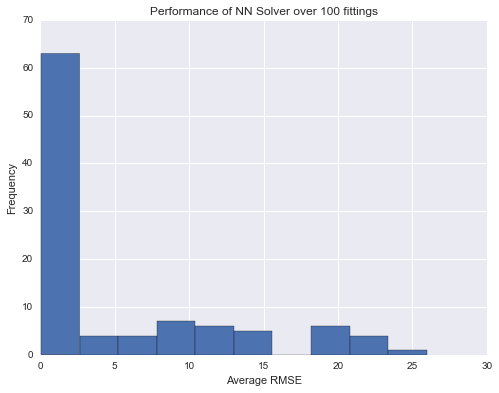
\includegraphics[width=0.7\textwidth]{VDP_DIst.png}
      \caption{Running NN solver 100 times to see the performance histogram \label{fig:VDP_perf_dist}}
\end{figure}

Since the fitting is satisfactory, we run the same fitting over 100 times to ensure reproducibility. From Fig. ~\ref{fig:VDP_perf_dist}, 76\% of the fittings result in relatively good fitting with average RMSE of less than 3.2.

Please refer to Van\_der\_Pol\_oscillator.ipynb for the code and visualizations of this section.

\subsection{Unstable, chaotic ODEs}

\subsubsection{Rössler Attractor}

Introduction

Mathematics

Results Discussion



\subsection{Stiff ODE system}


\subsection{Flexible initial conditions}


\section{Conclusions}

Limitation: $t$ cannot be every large; ANN has trouble fitting fast-oscillating solutions.

\section{Reference}

 % ------ bibliography -------
\begin{thebibliography}{99}

\bibitem{Hornik89}
Hornik, Kurt, Maxwell Stinchcombe, and Halbert White. "Multilayer feedforward networks are universal approximators." Neural networks 2.5 (1989): 359-366.
\bibitem{Lagaris98}
Lagaris, Isaac E., Aristidis Likas, and Dimitrios I. Fotiadis. "Artificial neural networks for solving ordinary and partial differential equations." IEEE Transactions on Neural Networks 9.5 (1998): 987-1000.
\bibitem{REF1}
https://en.wikipedia.org/wiki/Lotka-Volterra\_equations
\bibitem{REF2}
http://www.math.harvard.edu/library/sternberg/slides/11809LV.pdf
\bibitem{REF3}
http://people.kzoo.edu/barth/math280/articles/3speciesLV.pdf
\bibitem{REF4}
http://www2.me.rochester.edu/courses/ME406/webexamp5/vanpol.pdf
\bibitem{REF5}
Kaplan, D. and Glass, L., Understanding Nonlinear Dynamics, Springer, 240–244, (1995).

\end{thebibliography}

\end{document}